%-------------------- ĆWICZENIA --------------------
\section{Ćwiczenia 25-V-2017}

Wszędzie obowiązuje domyślne założenie, że wszystkie zmienne występujące w zagadnieniach programowania liniowego mogą przyjmować tylko wartości nieujemne.
\subsection{Ściąga}
\begin{description}
\item[$\beta $] $\rightarrow$ wielkość największego skojarzenia w grafie - ile jest skojarzeń.
\item[$\beta ^\star$] $\rightarrow$ maksimum funkcji $\sum _{e\in E(G)} x_e$ takie że $\sum _{e:v\in e} x_e\leq 1$ dla każdego $v \in V (G)$.
\item[$\gamma $] $\rightarrow$ minimalna liczba pokryciowa i najmniejsza liczba wierzchołków by mieć połączone ,,wszystkie'' krawędzie.
\item[$\gamma ^\star$] $\rightarrow$ minimum funkcji $\sum _{v\in V(G)} x_v$ takie że $\sum _{v:v\in e} x_v \geq 1$ dla każdego $e \in E(G)$.
\item[$\omega $] $\rightarrow$ liczba klikowa wyjaśniona na górze. 
\item[$\omega ^\star$] $\rightarrow$ maksimum funkcji $\sum _{v\in V(G)} x_v$ takie że $\sum _{v:v\in I} x_v \leq 1$ dla każdego zbioru niezależnego $I \subseteq V(G)$.
\item[$\chi $] $\rightarrow$ liczba chromatyczna - czyli ile kolorków muszą użyć by pomalować graf w taki sposób, aby żadne połączone dwa wierzchołki nie miały tego samego koloru.
\item[$\chi ^\star$] $\rightarrow$ minimum funkcji $\sum _{I\subseteq V(G)} x_I$ takie że $\sum _{I:v\in I} x_I \geq 1$ dla każdego $v \in V(G)$, przy czym w obu sumowaniach występują tylko zbiory niezależne. 
\end{description}

\subsection{Zadania domowe A}
\paragraph{A1} Sformułuj zagadnienia dualne do podanych poniżej. Nie rozwiązuj problemów.\\
\begin{minipage}{.5\textwidth}
\textbf{Problem 1} Zminimalizować funkcję
$$f(x, y, z) = z - x + y$$
dla zmiennych $x, y, z$ spełniających warunki:
$$\left\{\begin{matrix}
-x &+ 2y &- z &\geq -1\\
&-y &+z &\geq \sfrac{3}{2}
\end{matrix}\right.$$
\begin{align*}
&\begin{matrix}
y_1: & -x&+2y&-z&\geq 1\\
y_2:& &-y&+z&\geq\frac{3}{2}
\end{matrix}\\
&g(y_1,y_2)=-1y_1+\frac{3}{2}y_2\\
&\left\{\begin{matrix}
-y_1 &&\leq -1\\
2y_1&-y_2&\leq 1\\
-y_1&+y_2&\leq 1
\end{matrix}\right.\\
&\min _{x,y,z}f(x,y,z)=\max _{y_1,y_2} g(y_1,y_2)
\end{align*}
\end{minipage}%
\begin{minipage}{.5\textwidth}
\textbf{Problem 2} Zmaksymalizować funkcję
$$f(x, y, z, w) = x - y$$
dla zmiennych $x, y, z$, w spełniających warunki:
$$\left\{\begin{matrix}
x +&&& w &\leq 1\\
x -& y &&- \sfrac{1}{4}w &\leq 0\\
x -&2y +& z +&w &\leq 2
\end{matrix}\right.$$
\begin{align*}
&\begin{matrix}
y_1: & x &+ 	&	& w	&\leq  1\\
y_2: & x &- y  	&	&- \sfrac{1}{4} w &\leq 0\\
y_3: & x &- 2y 	&+z	&+w	&\leq 2
\end{matrix}\\
&g(y_1,y_2,y_3)=y_1+2y_3\\
&\left\{\begin{matrix}
y_1 &+ y_2 &+ y_3 &\geq 1\\
&-y_2 & -2y_2 &\geq -1\\
&&y_3 &\geq 0\\
y_1 &- \sfrac{1}{4} y_2 &+ y_3 &\geq 0
\end{matrix}\right.\\
&\max _{x,y,z,w} f(x,y,z,w)=\min _{y_1,y_2,y_3} (y_1,y_2,y_3)
\end{align*}
\end{minipage}

\paragraph{A2} Czy drugi problem jest dualny do pierwszego problemu, sformułowanego jako zagadnienie programowania liniowego? Rozwiąż (zdroworozsądkowo) oba problemy.

\begin{minipage}{.5\textwidth}
\textbf{Problem 1} Zmaksymalizować funkcję
$$f(x, y, z) = x - 2y$$
dla zmiennych $x, y, z$ spełniających warunki:
$$\left\{\begin{matrix}
x &+ y &&\leq 1\\
&-y &+ z &\leq \frac{1}{2}
\end{matrix}\right.$$
\begin{align*}
&\begin{matrix}
y_1: & x_1 &+x_2& &\leq 1\\
y_2: & &-x_2&+x_3 &\leq \sfrac{1}{2}
\end{matrix}\\
&g(y_1,y_2)=y_1+\frac{1}{2}y_2\\
&\left\{\begin{matrix}
y_1&&\geq 1\\
y_2&-y_2&\geq -2
\end{matrix}\right.\\
&\max _{x,y,z}f(x,y,z)=\min _{y_1,y_2}g(y_1,y_2)
\end{align*}
\end{minipage}%
\begin{minipage}{.5\textwidth}
\textbf{Problem 2} Zminimalizować funkcję
$$g(x, y) = x - \frac{1}{2}y$$
dla zmiennych $x, y$ spełniających warunki:
$$\left\{\begin{matrix}
x &&\geq 1\\
x &- y &\geq -2\\
&y &\geq 0
\end{matrix}\right.$$
\begin{align*}
&\begin{matrix}
y_1: & x_1 & &\geq 1\\
y_2: & x_1 &-x_2 &\geq -2\\
y_3: & & x_2 &\geq 0
\end{matrix}\\
&f(y_1,y_2,y_3)=y_1-2y_2\\
&\left\{\begin{matrix}
y_1	&+y_2	&		&\leq 1\\
	&-y_2	&+y_3	&\leq \frac{1}{2}
\end{matrix}\right.\\
&\min _{x,y}g(x,y)=\max _{y_1,y_2,y_3}f(y_1,y_2,y_3)
\end{align*}
\end{minipage}




\paragraph{A3} Dla podanych grafów (z pewnymi funkcjami zdefiniowanymi na zbiorze wierzchołków lub krawędzi) uzasadnij
prawdziwość podanych oszacowań na parametry $\beta ^\star, \gamma ^\star, \chi ^\star, \omega ^\star$. (Parametry te zdefiniowane były na wykładzie.)

\begin{enumerate}[label=\alph*)]
\item $\beta ^\star \geq 2$ 
\begin{figure}[H]
\centering
\begin{tikzpicture}[shorten >=1pt, auto, node distance=3cm, ultra thick,main node/.style={circle,draw,minimum size=.4cm,inner sep=0pt]}]%fill=black,
\begin{scope}%[every node/.style={font=\sffamily\Large\bfseries}]%[main node]
\node[main node] (v1) at (0,0) {1};
\node[main node] (v2) at (3,0) {2};
\node[main node] (v3) at (2.6,1) {3};
\node[main node] (v4) at (-.4,2) {4};
\node[main node] (v5) at (1.5,3) {5};
\end{scope}
\begin{scope}[every edge/.style={draw=black,ultra thick}]
\draw  (v1) edge node{$\sfrac{1}{2}$} (v2);
\draw  (v1) edge node{$\sfrac{1}{4}$} (v3);
\draw  (v1) edge node{$\sfrac{1}{4}$} (v4);
\draw  (v2) edge node{$\sfrac{1}{4}$} (v3);
\draw  (v3) edge node{$\sfrac{1}{4}$} (v4);
\draw  (v3) edge node{$\sfrac{1}{4}$} (v5);
\draw  (v4) edge node{$\sfrac{1}{4}$} (v5);
\end{scope}
\end{tikzpicture}
\end{figure}

$\beta ^\star$ $\rightarrow$ maksimum funkcji $\sum _{e\in E(G)} x_e\ t$ że $\sum _{e:v\in e} x_e\leq 1$ dla każdego $v \in V (G)$.
\begin{align*}
&\begin{matrix}
1: &\frac{1}{2}+\frac{1}{4}+\frac{1}{4}=1\\
2: &\frac{1}{2}+\frac{1}{4}=\frac{3}{4}\\
3: &\frac{1}{4}+\frac{1}{4}+\frac{1}{4}=\frac{3}{4}\\
4: &\frac{1}{4}+\frac{1}{4}+\frac{1}{4}=\frac{3}{4}\\
5: &\frac{1}{4}+\frac{1}{4}=\frac{1}{2}
\end{matrix}
\end{align*}
$$\beta ^\star =\frac{1}{4}+\frac{1}{4}+\frac{1}{4}+\frac{1}{4}+\frac{1}{4}+\frac{1}{4}+\frac{1}{2}=2$$

\item $\gamma ^\star \leq 2,5$
\begin{figure}[H]
\centering
\begin{tikzpicture}[shorten >=1pt, auto, node distance=3cm, ultra thick,main node/.style={circle,draw,minimum size=.1cm,inner sep=0pt]}]%,fill=black
\begin{scope}%[every node/.style={font=\sffamily\Large\bfseries}]%[main node]
\node[main node] (v1) at (0,0)[label=below:$\sfrac{1}{2}$] {1};
\node[main node] (v2) at (3,0)[label=below:$\sfrac{1}{2}$] {2};
\node[main node] (v3) at (3,3)[label=above:$\sfrac{1}{2}$] {3};
\node[main node] (v4) at (0,3)[label=left:$\sfrac{3}{4}$] {4};
\node[main node] (v5) at (-2,4.5)[label=above:$\sfrac{1}{4}$] {5};
\end{scope}
\begin{scope}[every edge/.style={draw=black,ultra thick}]
\draw  (v1) edge (v2);
\draw  (v1) edge (v4);
\draw  (v2) edge (v3);
\draw  (v3) edge (v4);
\draw  (v4) edge (v5);
\end{scope}
\end{tikzpicture}
\end{figure}
$\gamma ^\star$ $\rightarrow$ minimum funkcji $\sum _{v\in V(G)} x_v\ t$ że $\sum _{v:v\in e} x_v \geq 1$ dla każdego $e \in E(G)$.
\begin{align*}
&\begin{matrix}
1\leftrightarrow 2: & \frac{1}{2}+\frac{1}{2}=1\\
1\leftrightarrow 4: & \frac{1}{2}+\frac{3}{4}=\frac{5}{4}\\
2\leftrightarrow 1: & \frac{1}{2}+\frac{1}{2}=1\\
2\leftrightarrow 3: & \frac{1}{2}+\frac{1}{2}=1\\
3\leftrightarrow 2: & \frac{1}{2}+\frac{1}{2}=1\\
3\leftrightarrow 4: & \frac{1}{2}+\frac{3}{4}=\frac{5}{4}\\
4\leftrightarrow 1: & \frac{3}{4}+\frac{1}{2}=\frac{5}{4}\\
4\leftrightarrow 3: & \frac{3}{4}+\frac{1}{2}=\frac{5}{4}\\
4\leftrightarrow 5: & \frac{3}{4}+\frac{1}{4}=1
\end{matrix}
&\gamma ^\star = \frac{1}{4}+\frac{3}{4}+\frac{1}{2}+\frac{1}{2}+\frac{1}{2}=2.5
\end{align*}



\item $\omega ^\star \geq 3$
\begin{figure}[H]
\centering
\begin{tikzpicture}[shorten >=1pt, auto, node distance=3cm, ultra thick,main node/.style={circle,draw,minimum size=.1cm,inner sep=0pt]}]%fill=black,
\begin{scope}%[every node/.style={font=\sffamily\Large\bfseries}]%[main node]
\node[main node] (v1) at (0,0)[label=below:$1$] {1};
\node[main node] (v2) at (3,0)[label=below:$\sfrac{1}{2}$] {2};
\node[main node] (v3) at (3,3)[label=above:$1$] {3};
\node[main node] (v4) at (0,3)[label=above:$\sfrac{1}{2}$] {4};
\end{scope}
\begin{scope}[every edge/.style={draw=black,ultra thick}]
\draw  (v1) edge (v2);
\draw  (v1) edge (v4);
\draw  (v1) edge (v3);
\draw  (v2) edge (v3);
\draw  (v3) edge (v4);
\end{scope}
\end{tikzpicture}
\end{figure}
$\omega ^\star$ $\rightarrow$ maksimum funkcji $\sum _{v\in V(G)} x_v$ takiej że $\sum _{v:v\in I} x_v \leq 1$ dla każdego zbioru niezależnego $I \subseteq V(G)$.
$$\{\underset{\sfrac{1}{2}}{\{4,2\}},\underset{1}{\{1\}},\underset{\sfrac{1}{2}}{\{2\}},\underset{1}{\{3\}},\underset{\sfrac{1}{2}}{\{4\}}\}$$
$$\omega ^\star = 3$$
$$\chi (G)\geq \chi ^\star (G)=\omega ^\star (G)\geq\omega (G)$$
$\chi (G) =3\ \ \omega (G) =3$
\end{enumerate}


\paragraph{A4}
\begin{itemize}
\item Czy dla grafu (a) z poprzedniego zadania zachodzi $\gamma ^\star \geq 2$ ?

\textbf{Odpowiedz: }Wynika z twierdzenia o dualnoci: 
$$\gamma (G) \geq \gamma ^\star (G)=\beta ^\star (G)\geq \beta (G)$$
Więc tak zachodzi
\item Czy dla grafu (b) z poprzedniego zadania zachodzi $\beta ^\star > 2,5$ ?

\textbf{Odpowiedź: }Jak wyżej - nie bangla
\item Czy dla grafu (c) z poprzedniego zadania zachodzi $\chi ^\star = 3$ ?

\textbf{Odpowiedź: }
$$\chi (G)\geq \chi ^\star(G)=\omega ^\star(G)\geq \omega (G)$$
więc tak.
\end{itemize}


\paragraph{A5} Niech $G$ będzie grafem (c) z zadania A3.
\begin{enumerate}[label=\alph*)]
\item Wypisz wszystkie pięć zbiorów niezależnych grafu $G$.

\textbf{Odpowiedź:}
$$\{\{2,4\},\{1\},\{2\},\{3\},\{4\}\}$$
\item Każdemu zbioru niezależnemu $I \subseteq V(G)$ przyporządkuj liczbę nieujemną $y_I$ w taki sposób, by dla każdego wierzchołka w zachodził warunek $\sum _{I:w \in I}y_I \geq 1$ (sumujemy po zbiorach niezależnych).
$$\{\underset{0.5}{\{2,4\}},\underset{1}{\{1\}},\underset{0.5}{\{2\}},\underset{1}{\{3\}},\underset{0.5}{\{4\}}\}$$
\item Jakie z tego wynika oszacowanie na $\chi ^\star$?

$$\chi ^\star = \sum y_I=3.5$$
\item Jakie z tego wynika oszacowanie na $\omega ^\star$?

Z twierdzenia o dualności wynika, że $\omega ^\star (G) = \chi ^\star (G)$
\end{enumerate}

\paragraph{A6} Dla podanych grafów:\\
\begin{minipage}{.5\textwidth}
a)
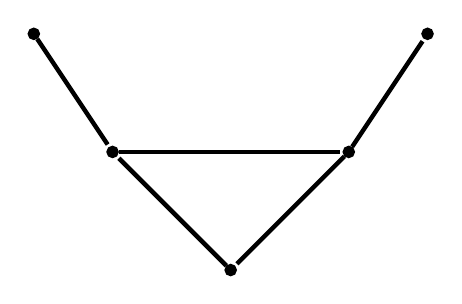
\begin{tikzpicture}[shorten >=1pt, auto, node distance=3cm, ultra thick,main node/.style={circle,fill=black,draw,minimum size=.1cm,inner sep=0pt]}]
\node[main node] (v1) at (0,0) {};
\node[main node] (v2) at (-1.5,1.5) {};
\node[main node] (v3) at (1.5,1.5) {};
\node[main node] (v5) at (-2.5,3) {};
\node[main node] (v4) at (2.5,3) {};
\draw  (v1) edge (v2);
\draw  (v2) edge (v3);
\draw  (v3) edge (v1);
\draw  (v3) edge (v4);
\draw  (v5) edge (v2);
\end{tikzpicture}
\end{minipage}%
\begin{minipage}{.5\textwidth}
b)
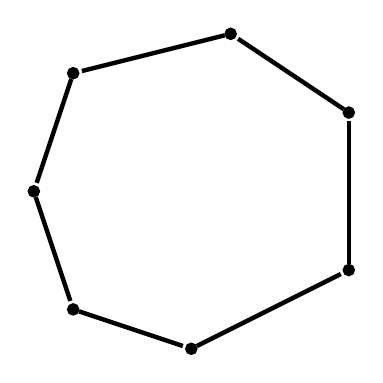
\begin{tikzpicture}[shorten >=1pt, auto, node distance=3cm, ultra thick,main node/.style={circle,fill=black,draw,minimum size=.1cm,inner sep=0pt]}]
\node[main node] (v1) at (0,0) {};
\node[main node] (v2) at (2,1) {};
\node[main node] (v3) at (2,3) {};
\node[main node] (v4) at (0.5,4) {};
\node[main node] (v5) at (-1.5,3.5) {};
\node[main node] (v6) at (-2,2) {};
\node[main node] (v7) at (-1.5,0.5) {};
\draw  (v1) edge (v2);
\draw  (v2) edge (v3);
\draw  (v3) edge (v4);
\draw  (v4) edge (v5);
\draw  (v5) edge (v6);
\draw  (v6) edge (v7);
\draw  (v7) edge (v1);
\end{tikzpicture}
\end{minipage}
\begin{itemize}
\item Wyznacz liczbę chromatyczną $\chi$, liczbę klikową $\omega$, przykładowe najmniejsze pokrycie wierzchołkowe, i przykładowe największe skojarzenie.
\item Oszacuj jak najlepiej potrafisz z góry i z dołu parametry $\beta ^\star, \gamma ^\star, \omega ^\star, \chi ^\star$.
\end{itemize}
\begin{enumerate}[label=\alph*)]
\item $\chi = 3\ \ \omega = 3\ \ \gamma = 2\ \ \beta = 2$
\item $\chi = 3\ \ \omega = 2\ \ \gamma = 4\ \ \beta = 3$
\end{enumerate}
\begin{enumerate}[label=\alph*)]
\item $\chi ^\star\leq 3\ \ \omega ^\star\geq 3\ \ \gamma ^\star\leq 2\ \ \beta ^\star\geq 2$
\item $\chi ^\star\leq 3\ \ \omega ^\star\geq 2\ \ \gamma ^\star\leq 4\ \ \beta ^\star\geq 3$
\end{enumerate}

\paragraph{A7} Oceń poprawność każdego z poniższych zdań. W każdym przypadku poprzyj odpowiedź, w zależności od potrzeby, uzasadnieniem ogólnym, przykładem lub kontrprzykładem.
\begin{enumerate}[label=\alph*)]
\item Dla każdego grafu $G$ moc największego skojarzenia jest nie większa niż $\beta ^\star(G)$.

$$\forall _{G} \beta (G) \not > \beta ^\star (G)$$
\textbf{Odpowiedź: }Z faktu na wykładzie wiemy, że $\beta ^\star (G)\geq \beta (G)$ więc, jest to \textbf{PRAWDA}
\item Dla każdego grafu $G$ moc najmniejszego pokrycia wierzchołkowego jest nie mniejsza niż $\gamma ^\star(G)$.

$$\forall _G \gamma (G) \not < \gamma ^\star(G)$$
\textbf{Odpowiedź: }Z faktu podanego, że $\gamma (G)\geq \gamma ^\star(G)$ wynika, że jest to \textbf{PRAWDA}
\item W każdym grafie ułamkowa liczba skojarzenia jest równa ułamkowej liczbie pokryciowej.

$$\forall _G \beta ^\star (G)=\gamma ^\star (G)$$
\textbf{Odpowiedź: }Z faktu podanego na wykładzie, że $\gamma (G) \geq \gamma ^\star (G)=\beta ^\star (G)\geq \beta (G)$ wynika, że podaje zdanie jest \textbf{PRAWDZIWE}
\item W każdym grafie moc największego skojarzenia jest równa mocy najmniejszego pokrycia.

$$\forall _G \beta (G)=\gamma (G)$$
\textbf{Odpowiedź: }Z faktu podanego na wykładzie, że $\gamma (G) \geq \gamma ^\star (G)=\beta ^\star (G)\geq \beta (G)$ wynika, że podaje zdanie jest \textbf{NIEPRAWDZIWE} 
\begin{figure}[H]
\centering
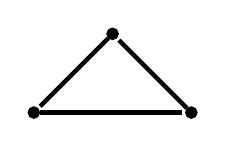
\begin{tikzpicture}[shorten >=1pt, auto, node distance=3cm, ultra thick,main node/.style={circle,fill=black,draw,minimum size=.1cm,inner sep=0pt]}]
\node[main node] (v1) at (0,0) {};
\node[main node] (v2) at (2,0) {};
\node[main node] (v3) at (1,1) {};
\draw  (v1) edge (v2);
\draw  (v2) edge (v3);
\draw  (v3) edge (v1);
\end{tikzpicture}
\caption*{$\beta = 1\ \gamma =2$}
\end{figure}
\item W każdym grafie ułamkowa liczba klikowa jest równa ułamkowej liczbie chromatycznej.

$$\forall _G\omega ^\star (G)=\chi ^\star (G)$$
\textbf{Odpowiedź: }Z faktu podanego na wykładzie, że $\chi (G)\geq \chi ^\star(G)=\omega ^\star(G)\geq \omega (G)$ wynika, że podane zdanie jest \textbf{PRAWDZIWE}.
\item W każdym grafie moc największej kliki jest równa liczbie chromatycznej.

$$\forall _G \omega (G)=\chi (G)$$
\textbf{Odpowiedź: }Z faktu podanego na wykładzie, że $\chi (G)\geq \chi ^\star(G)=\omega ^\star(G)\geq \omega (G)$ wynika, że podane zdanie \textbf{NIE JEST PRAWDZIWE}
\begin{figure}[H]
\centering
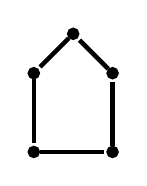
\begin{tikzpicture}[shorten >=1pt, auto, node distance=3cm, ultra thick,main node/.style={circle,fill=black,draw,minimum size=.1cm,inner sep=0pt]}]
\node[main node] (v1) at (0,0) {};
\node[main node] (v2) at (1,0) {};
\node[main node] (v3) at (1,1) {};
\node[main node] (v4) at (0.5,1.5) {};
\node[main node] (v5) at (0,1) {};
\draw  (v1) edge (v2);
\draw  (v2) edge (v3);
\draw  (v3) edge (v4);
\draw  (v4) edge (v5);
\draw  (v5) edge (v1);
\end{tikzpicture}
\caption*{$\omega = 2\ \chi =3$}
\end{figure}
\end{enumerate}

\subsection{Zadania domowe B}
\paragraph{B1} Przypuśćmy, że chcemy Zminimalizować funkcję
$f(x, y, z, w, u) = w - u$,
przy ograniczeniach zadanych nierównościami obok. Użyj dualności i sprowadź ten problem do równoważnego mu problemu maksymalizacji odpowiedniej funkcji. Nie rozwiązuj problemu.
$$\left\{\begin{matrix}
-x &- 2y &- z &- 3w &+ u &\geq 0\\
-2x &- y &- 2z &&+ u&\geq 0\\
&-2y &- z &- 2w &+ u &\geq 0\\
-x &&- 2z &- w &+ u &\geq 0\\
-2x &- 2y &- 2z &- 2w &+ u &\geq 0\\
x &+ y &+ z &+ w &&\geq 1 \end{matrix}\right.$$


\paragraph{B2} Dobra wróżka powiedziała, że podana funkcja $f_1$ na obszarze ograniczonym podanymi nierównościami osiąga minimum dla $(x; y; z; u) = (0; 0; 0,29; 0,22)$. Czy na tej podstawie potrafisz wyznaczyć, jaka jest największą wartość funkcji $f_2$ przy podanym poniżej niej ograniczeniach?

\begin{minipage}{.5\textwidth}
$$\left\{\begin{matrix}
f_1(x, y, z, u) = 16x + 8y + 8z\\
4x - 8y + 9u \geq 2\\
6x + 4y + 7z - 9u \geq 0\\
y + 5z + 2u \geq -5\\
\end{matrix}\right.$$
\end{minipage}%
\begin{minipage}{.5\textwidth}
$$\left\{\begin{matrix}
f_2(x, y, z) = 2x - 5z\\
4x + 6y \leq 16\\
-8x + 4y + z \leq 8\\
7y + 5z \leq 8\\
9x - 9y + 2z \leq 0\\
\end{matrix}\right.$$
\end{minipage}



\paragraph{B3} Przypuśćmy, że chcemy Zmaksymalizować funkcję
$f(x, y) = x - 3y$ przy podanych obok ograniczeniach.
\begin{enumerate}[label=\alph*)]
\item Sformułuj zagadnienie dualne do powyższego.
\item Wyznacz szukane maksimum funkcji $f$ i minimum funkcji z zagadnienia dualnego.
\end{enumerate}
$$\left\{\begin{matrix}
x &- y &\leq -1\\
x &&\leq 2\\
-2x&+ y &\leq 3\\
\end{matrix}\right.$$

\paragraph{B4} Oszacuj jak najlepiej potrafisz $\chi ^\star(G)$, z góry i z dołu, gdy $G$ jest cyklem na trzynastu wierzchołkach.

\paragraph{B5} Oszacuj jak najlepiej potrafisz $\beta ^\star, \gamma ^\star \text{ i } \chi ^\star(G)$, z góry i z dołu, gdy
\begin{enumerate}[label=\alph*)]
\item  $G$ jest grafem powstałym z cyklu na trzynastu wierzchołkach, przez dodanie do niego krawędzi łączących wierzchołki posiadające wspólnego sąsiada (czyli dodajemy 13 krawędzi).
\item  $G = K_{3,5}$.
\end{enumerate}


\subsection{Zadania na ćwiczeniach}
\paragraph{Zad.1} Rozwiąż podane zagadnienie programowania liniowego i zagadnienie do niego dualne.
$$\left\{\begin{matrix}
f(x_1, x_2, x_3) = x_1 + 2x_2 (max)\\
x_1 + x_2 + x_3 \leq 2\\
2x_2 - x_3 \leq 1
\end{matrix}\right.$$

\paragraph{Zad.2}
\begin{enumerate}[label=\alph*)]
\item Oblicz $\beta ^\star (G)$  i $\gamma ^\star (G)$, dla podanych grafów.
\item Podaj rozwiązania dla odpowiadających tym parametrom zagadnień programowania liniowego (jakie liczby wierzchołkom/krawędziom przyporządkować?)
\end{enumerate}


\paragraph{Zad.3}
\begin{enumerate}[label=\alph*]
\item Oblicz $\omega ^\star (G)$ i $\chi ^\star (G)$, dla podanych grafów.
\item Podaj rozwiązania dla odpowiadających tym parametrom zagadnień programowania liniowego (jakie liczby wierzchołkom/zbiorom niezależnym przyporządkować?)
\end{enumerate}

\paragraph{Zad.4}
\begin{enumerate}
\item Sformułuj zagadnienie programowania całkowitoliczbowego, znajdujące liczbę niezależności $\alpha (G)$ grafu.
\item Sformułuj zagadnienie programowania liniowego, znajdujące ułamkową liczbę niezależności $\alpha ^\star(G)$ grafu.
\item Sformułuj zagadnienie dualne do poprzedniego. Z jakiem parametrem grafowym jest związane?
\end{enumerate}



%-------------------- WYKŁAD --------------------
\section[Wykład 13: 8-VI-2017 - Temat: Ekspandery]{Temat: Ekspandery}
\begin{definition}[Ekspander]
Ekspander to graf w którym najmniejsza niezerowa wartość własna Laplasjanu leży daleko od zera.\\
EKSPANDER $\rightarrow$ graf o równomiernie rozłożonych krawędziach
\end{definition}
\begin{figure}[H]
\centering
\begin{tikzpicture}
\coordinate (A) at (0.45,0);
\coordinate (B) at (1.5,0);
\coordinate (D) at (3.5,0);
\coordinate (E) at (6.5,0);

\draw[->] (0,0) -- (7,0);

\draw[thick] ($(A)+(0,5pt)$) node[above] {$0$} -- ($(A)-(0,5pt)$);
\draw[thick] ($(B)+(0,5pt)$) node[above] {$\lambda _1$} -- ($(B)-(0,5pt)$);
\draw[thick] ($(D)+(0,5pt)$) node[above] {Wartości własne} -- ($(D)-(0,5pt)$);
\draw[thick] ($(E)+(0,5pt)$) node[above] {$2d$} -- ($(E)-(0,5pt)$);
\draw[decorate,decoration={brace,amplitude=5pt,mirror,raise=3mm}] (A) -- (B) node [black,midway,yshift=-7mm] {\footnotesize $\epsilon d$};
\end{tikzpicture}
\end{figure}

\subsection{Zastosowanie ekspanderów}
\subsubsection{Teoria kodów}
\paragraph{Kody Spiser - Spielman} wymyślone przez: M. Spiser D. Spielman
\begin{figure}[H]
\centering
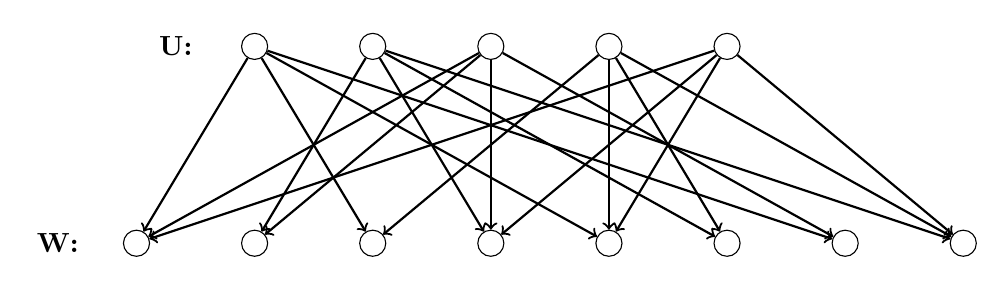
\begin{tikzpicture}
\tikzstyle{arrow}=[->, draw, thick]
\node[draw, circle] (v3) at (0,0) {};
\node[draw, circle] (v6) at (-4.5,-2.5) {};
\node[draw, circle] (v10) at (-3,-2.5) {};
\node[draw, circle] (v7) at (-1.5,-2.5) {};
\node[draw, circle] (v11) at (0,-2.5) {};
\node[draw, circle] (v8) at (1.5,-2.5) {};
\node[draw, circle] (v12) at (3,-2.5) {};
\node[draw, circle] (v9) at (4.5,-2.5) {};
\node[draw, circle] (v13) at (6,-2.5) {};
\node[draw, circle] (v2) at (-1.5,0) {};
\node[draw, circle] (v4) at (1.5,0) {};
\node[draw, circle] (v1) at (-3,0) {};
\node[draw, circle] (v5) at (3,0) {};
\node (v0) at (-4,0) {\textbf{U:}};
\node (v00) at (-5.5,-2.5) {\textbf{W:}};
    
\draw[arrow]  (v1) edge (v6);
\draw[arrow]  (v1) edge (v7);
\draw[arrow]  (v1) edge (v8);
\draw[arrow]  (v1) edge (v9);
\draw[arrow]  (v2) edge (v10);
\draw[arrow]  (v2) edge (v11);
\draw[arrow]  (v2) edge (v12);
\draw[arrow]  (v2) edge (v13);
\draw[arrow]  (v3) edge (v6);
\draw[arrow]  (v3) edge (v11);
\draw[arrow]  (v3) edge (v9);
\draw[arrow]  (v3) edge (v10);
\draw[arrow]  (v4) edge (v7);
\draw[arrow]  (v4) edge (v12);
\draw[arrow]  (v4) edge (v13);
\draw[arrow]  (v4) edge (v8);
\draw[arrow]  (v5) edge (v6);
\draw[arrow]  (v5) edge (v13);
\draw[arrow]  (v5) edge (v11);
\draw[arrow]  (v5) edge (v8);
\end{tikzpicture}
\end{figure}
$$\bbordermatrix{
&\Huge U &\Huge W\cr
\Huge U& \Huge O &\Huge H\cr
\Huge W & \Huge H^T & \Huge O 
}$$
Przypuśćmy, że graf $G$ jest ekspanderem.\\
Wtedy bardzo szybko można skorygować 2 błędy.
\begin{description}
\item[$U_1$] $|U|=100$, każdy wierzchołek $U$ jest połączony z 20 wierzchołkami z $W$
\item[$W_1$] $|W|=1000$
\end{description}
Taki graf (jeśli jest ekspanderem) potrafi skorygować nawet $5\%$ błędów.

\subsubsection{Liczenie średniej odległości}
\begin{theorem}[Metatwerdzenie]
Ekspander to rzadki graf który często ,,zachowuje się'' jak pełny.
\end{theorem}
\begin{proof}
Przypuśćmy, że mamy $n=10^5$ punktów, który jest ekspanderem.\\
Średnia odległość liczona po krawędziach tego grafu przybliża bardzo dobrze średnią odległość w liczonym grafie.
\end{proof}

\subsubsection{,,Zmniejszenie prawdopodobieństwa''}
\begin{theorem}[Małe twierdzenie Fermata]
$$a^{p-1}\equiv 1 (\mod p)$$
\end{theorem}
Przypuśćmy, że $n$ jest liczbą złożoną
$$a^{n-1}\equiv 1(\mod m)$$
dla co najwyżej potęgi liczb całkowitej produktu $[1;n-1]$
\begin{figure}[H]
\centering 
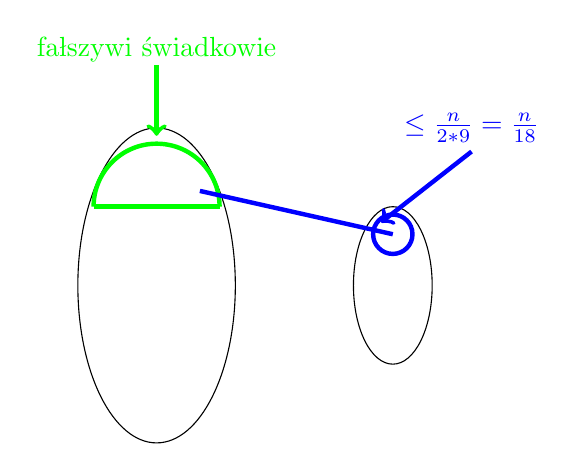
\begin{tikzpicture}
\draw  (0,0) ellipse (1 and 2);
\draw  (3,0) ellipse (.5 and 1);
\draw[ultra thick,color=green] (.8,1) arc (0:180:.8cm);
\draw[ultra thick,color=green] (-.8,1) -- (.8,1);
\node[color=green] at (0,3) {fałszywi świadkowie};
\draw[->,ultra thick,color=green] (0,2.8) -- (0,1.9);
\draw[ultra thick,color=blue]  (3,.65) ellipse (.25 and .25);
\draw[ultra thick,color=blue] (.55,1.2) -- (3,.65);
\node[ultra thick,color=blue] at (4,2) {$\leq \frac{n}{2*9}=\frac{n}{18}$};
\draw[->,ultra thick,color=blue] (4,1.7) -- (2.85,.8);
\end{tikzpicture}
\end{figure}
$d=10$ $|S|\leq \frac{n}{19}$ $|N(S)|> 9|S|$

I tak zamiast $\binom{1}{2}^k$ uzyskujemy $\binom{1}{19}^k$ 

%----------------------------------------------------------------

\section{Rozgrzewka przed kolokwium I}
\paragraph{Zad.1}
Proszę odpowiedzieć tak/nie z uzasadnieniem (ew. odpowiednim przykładem/kontrprzykładem).
\begin{enumerate}[label=\alph*)]
\item Czy dopełnienie każdego grafu $G$ niespójnego jest grafem spójnym?
\item Czy istnieje drzewo na $n \geq 5$ wierzchołkach, którego dopełnienie jest lasem?
\item  Czy jeśli graf $G$ posiada obchód Eulera, to graf krawędziowy grafu $G$ również ma obchód Eulera?
\item Czy niezawieranie $K_5$ jest własnością zamkniętą na branie minora? jeśli tak, to wskaż najmniejszy zbiór minorów zakazanych dla tej własności.
\item  Czy każdy $20$-regularny graf na $34$ wierzchołkach zawiera skojarzenie doskonałe?
\item Czy prawdą jest, że jeśli graf $G$ zawiera $K_5$ jako minor, to $\chi(G) \geq 5$?
\item  Czy istnieje graf regularny, którego spektrum (czyli ciągiem wszystkich wartości własnych) jest: $2, 2, -1, -1, -1, -1$ ?
\end{enumerate}


\paragraph{Zad.2} Załóżmy, że w macierzy binarnej $n\times n$ w każdym rzędzie i wierszu jest po $k$ jedynek ($1 \leq k \leq n$). Czy wynika z tego, że można pokolorować jedynki $k$ kolorami tak, aby żadne dwie jedynki tego samego koloru nie znajdowały się w tym samym rzędzie ani w tej samej kolumnie?

\paragraph{Zad.3} Graf $G$ o 212 wierzchołkach jest dopełnieniem grafu składającego się z 154 składowych, z których 4 to cykle o długości trzy, 50 to izolowane krawędzie, a pozostałe 100 to wierzchołki izolowane.\\
Znajdź liczbę chromatyczną grafu $G$.

\paragraph{Zad.4} Macierz przyległości $A$ pewnego grafu $G$ o 12 wierzchołkach spełnia równanie $A^2-A-2I = 0$.
\begin{enumerate}[label=\alph*)]
\item Wyznacz wszystkie wartości własne macierzy $A$ (wraz z krotnościami).
\item Ile krawędzi ma graf $G$ ?
\item Ile trójkątów ($K_3$) zawiera $G$ ?
\end{enumerate}


\paragraph{Zad.5} Czy można obejść każde pole poniższej szachownicy dokładnie raz i wrócić na miejsce startu? Zakładamy, że przechodzimy zawsze z pola na pole sąsiednie, czyli graniczące bokiem. Proszę podać interpretację grafową tego problemu, a następnie rozwiązać go.

\begin{figure}[H]
\centering
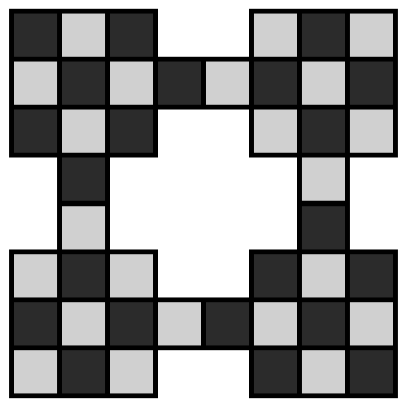
\includegraphics[width=.6\textwidth]{img/ROZ_1_5}
\end{figure}

\section{Rozgrzewka przed kolokwium II}
\paragraph{Zad.1} Złośliwa czarownica wymazała niektóre liczby z poniższego laplasjanu pewnego grafu (znaki ,,?''). Uzupełnij laplasjan i wyznacz liczbę drzew rozpiętych w tym grafie.
$$\begin{bmatrix}
3& ?& -1& -1\\
-1& ?& -1& ?\\
-1& ?& ?& -1\\
?& ?& -1& 2
\end{bmatrix}$$

\paragraph{Zad.2} Oto laplasjan $L$ pewnego grafu G, o którym wiadomo, że największej wartości własnej macierzy $L$ odpowiada wektor $(1, 1, 1, 1, 1, 1, -1, -1, -1, -1, -1, -1)$. Oszacuj z góry jak najlepiej potrafisz liczbę krawędzi w największym cięciu grafu $G$.

\begin{figure}[H]
\centering
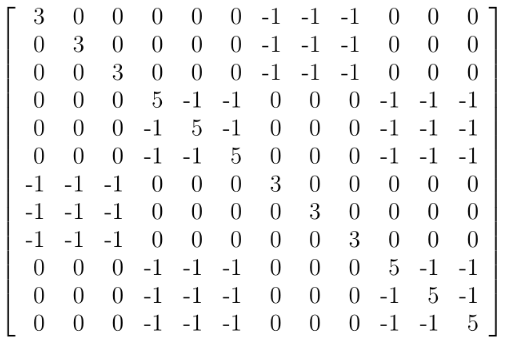
\includegraphics[width=.6\textwidth]{img/ROZ_2_2}
\end{figure}

\paragraph{Zad.3} Znajdź bazę ortonormalna, składającą się z wektorów własnych dla grafu $G$ na sześciu wierzchołkach o dwóch składowych, z których jedna to krawędź izolowana, a druga to $K_4$.

\paragraph{Zad.4} Wyznacz rozkład stacjonarny dla błądzenia po grafie, w którym w każdym kroku z wierzchołka $v$ przechodzimy do każdego z sąsiadów $v$ z prawdopodobieństwem $\sfrac{1}{\deg  (v)^2}$, a pozostajemy w miejscu z prawdopodobieństwem $1 - \sfrac{1}{\deg (v)}$. Fakt, że znaleziony przez Państwa rozkład jest stacjonarny, należy oczywiście uzasadnić.

\paragraph{Zad.5} Zaproponuj prosty algorytm, generujący za pomocą łańcucha Markowa las w grafie $G$ w taki sposób, że po wielu krokach otrzymamy w przybliżeniu każdy las $L$ z prawdopodobieństwem proporcjonalnym do $4^{|E(L)|}$. Poprawność algorytmu należy uzasadnić.

\paragraph{Zad.6} Tasujemy talię 3 kart $A$, $B$ i $C$, w następujący sposób: w każdym kroku wybieramy z jednakowym prawdopodobieństwem kartę środkową lub spodnią i przekładamy ją na wierzch talii. Skonstruuj łańcuch Markowa odpowiadający temu procesowi, wypisz macierz przejścia dla tego łańcucha i sprawdź czy
\begin{enumerate}[label=\alph*)]
\item jest on nieprzywiedlny i nieokresowy?
\item jest odwracalny?
\item posiada rozkład stacjonarny jednostajny?
\item posiada więcej niż jeden rozkład stacjonarny?
\end{enumerate}

\section{Rozgrzewka przed kolokwium III}
\paragraph{Zadanie 1} Skonstruuj odpowiednie sprzęgnięcie (coupling) pokazujące, że powolne błądzenie po $K_{n,n}$ szybko się miesza (tzn. należy oszacować z góry czas mieszania $\tau$ ). Przypominamy, że przy błądzeniu powolnym pozostajemy w wierzchołku $v$ z prawdopodobieństwem $\sfrac{1}{2}$, a przechodzimy do sąsiada $v$ z prawdopodobieństwem $\sfrac{1}{2\deg (v)}$.

\paragraph{Zadanie 2} Tasujemy talię $n$ różnych kart w następujący sposób : zaczynamy od dowolnego stosu, wybieramy losowo (z jednakowym prawdopodobieństwem) jedną z $n$ kart i kładziemy ją na wierzch. Chcemy uzasadnić, że odpowiadający takiemu tasowaniu łańcuch Markowa szybko się miesza i w tym celu definiujemy następujące sprzęgnięcie : Zaczynamy od dwóch różnych permutacji (stosów) naszej talii. W każdym kroku wybieramy losowo w sposób jednostajny kartę z pierwszego stosu, z drugiego stosu wyciągamy kartę taką samą a następnie w obu stosach wybraną kartę przekładamy na wierzch. Uzasadnij, analizując powyższe sprzęgnięcie, że czas mieszania $\tau$ łańcucha wynosi $O(n \log n)$, tzn. $\tau \leq cn \log n$ dla pewnej stałej $c > 0$.

\paragraph{Zadanie 3} Czy istnieje ciało $Q$, liczba naturalna $n$ i kod liniowy $C \subseteq Q^n$, który jest doskonały, ma rozstęp $3$ i składa się z $16$ wyrazów ($|C| = 16$) ? Jeżeli nie – uzasadnij, dlaczego. Jeżeli tak – podaj przykładową macierz generującą taki kod.

\paragraph{Zadanie 4} Oto macierz generująca pewnego kodu $C$ nad ciałem $\mathtt{Z}_3$ :
$$\begin{bmatrix}
1& 1& 1& 1& 2\\
2& 1& 2& 1& 0
\end{bmatrix}$$

Niech $\bar{y} = 11211 \in \mathtt{Z}^5_3$.
\begin{enumerate}[label=\alph*)]
\item Ile wyrazów z $\mathtt{Z}^5_3$
znajduje się w kuli Hamminga o promieniu $2$ i środku w $\bar{y}$?
\item Wyznacz macierz parzystości kodu $C$ i przy jej pomocy sprawdź, czy $\bar{y} \in C$.
\item Wyznacz wszystkie wyrazy $\bar{e}$ o tym samym indeksie co $\bar{y}$ o najmniejszej wadze (czyli będące w najmniejszej odległości Hamminga od $00000$). Jaka jest najmniejsza liczba współrzędnych, jakie musimy zmienić w $\bar{y}$, aby otrzymać wyraz kodu ?
\item Czy kod $C$ jest doskonały ?
\end{enumerate}

\paragraph{Zadanie 5} Przypuśćmy, że mamy zmaksymalizować funkcję $$f(x, y, z) = 2x - 3y$$ w obszarze, w którym $x + y \leq 23$, $x + y + 2z \leq 12$, $y + z \leq 4$, $3x + z \leq 15$. Zamień ten problem na równoważny problem dualny, dotyczący minimalizacji pewnej funkcji liniowej.

\paragraph{Zadanie 6} Fabryka czekolady produkuje różne smakołyki, podzielone na dwie główne kategorie: z czekolady białej i czekolady deserowej. Szef fabryki ma bazę $m$ klientów, dzięki której wie, jakie produkty kto kiedykolwiek kupił. Postanowił zbadać opinie klientów o $p$ produktach, wysyłając kwestionariusz do każdego z nich. Aby nie zniechęcać klientów do jego wypełnienia, kwestionariusz nie może być za długi. Szef przyjął zatem następujące założenia:
\begin{itemize}
\item nie można pytać o produkt, którego klient nigdy nie kupił;
\item produktów z czekolady białej, o które pytamy $i$– tego klienta, nie może być więcej niż $b_i$ (dla $i = 1, . . . , m$);
\item produktów z czekolady deserowej, o które pytamy $i$– tego klienta, nie może być więcej niż $d_i$ (dla $i = 1, . . . , m$);
\item aby badanie było wiarygodne, każdy produkt $j$ musi być oceniony przez co najmniej $k_j$ klientów.
\end{itemize}

Zakładamy, że dysponujemy tylko algorytmem znajdują cym największy przepływ i najmniejsze cięcie w sieciach z jednym źródłem i jednym ujściem. Jak rozstrzygnąć, czy przygotowanie takich kwestionariuszy jest możliwe? Odpowiedź powinna być dokładnie uzasadniona.

